\documentclass{article}
\usepackage[utf8]{inputenc}
\usepackage[english]{babel}
\usepackage{amsmath}
\usepackage[]{amsthm}
\usepackage[]{amssymb} 
\usepackage{mathrsfs}
\usepackage{tcolorbox}
\usepackage{nicefrac}
\usepackage{mathtools}
% \usepackage{graphicx}
\usepackage{caption}
\usepackage{subcaption}
\usepackage{array}

\graphicspath{ {./images/} }

\theoremstyle{definition}
\newtheorem*{claim}{Claim}
\newtheorem*{corollary}{Corollary}
\DeclareMathOperator{\adj}{\operatorname{adj}}
\DeclareMathOperator{\im}{\operatorname{im}}
\DeclareMathOperator{\spn}{\operatorname{span}}
\DeclareMathOperator{\nll}{\operatorname{null}}
\newcommand{\trace}{\operatorname{trace}}
\newcommand{\R}{\mathbb{R}}
\newcommand{\Z}{\mathbb{Z}}
\newcommand{\N}{\mathbb{N}}
\newcommand{\F}{\mathbb{F}}
\newcommand{\C}{\mathbb{C}}
\newcommand{\D}{\operatorname{D}}
\newcommand{\GL}{\operatorname{GL}}
\newcommand{\SL}{\operatorname{SL}}
\newcommand{\GLnR}{\GL_n(\R)}
\newcommand{\SLnR}{\SL_n(\R)}
\DeclarePairedDelimiter\floor{\lfloor}{\rfloor}
\DeclarePairedDelimiter\set{\{}{\}}
\DeclarePairedDelimiter\abs{\lvert}{\rvert}
\DeclarePairedDelimiter\genby{\langle}{\rangle}
\DeclarePairedDelimiter\bilform{\langle}{\rangle}
\newcommand{\restrict}[1]{ \big|_{#1} }
\newcommand{\evalat}[2]{\Big|_{#1}^{#2}}


\title{18.701: Problem Set 10}
\author{Dmitry Kaysin}
\date{August 2020}
\begin{document}
\maketitle 


\subsection*{Problem 1}

\begin{tcolorbox}
a) Let $\SL_2$ be the special linear group of real matrices with determinant $1$.
Determine the possible eigenvalues $\lambda$ (real or complex) of the elements of $\SL_2$, and make a drawing showing the points $\lambda$ in the complex plane.
\end{tcolorbox}

We start with $2 \times 2$ matrix of the form
\[
    A =
    \begin{pmatrix}
        a & b \\
        c & d
    \end{pmatrix}
\]
with $\det A = ad - bc = 1$.

Characteristic polynomial of $A$ is $t^2 - tr + 1$ where $r = \trace A = a+d$.
Eigenvalues of $A$ are thus
\[
    \lambda = \frac{r \pm \sqrt{r^2-4}}{2}.
\]
As $r \to \infty : \lambda \to \pm \infty$ and
as $r \to -\infty : \lambda \to \mp 0$.
For $r$ in the interval $(-\infty, -2] \cup [2, \infty)$ eigenvalues of $A$ are real.
For $r$ in the interval $(-2, 2)$ eigenvalues of $A$ are complex, occur in conjugate pairs and their locus is upper and lower half of the unit circle on the complex plane.

\begin{figure}[h]
    \caption{Possible eigenvalues of $A \in \SL_2$ in the complex plane.}
    \centering
    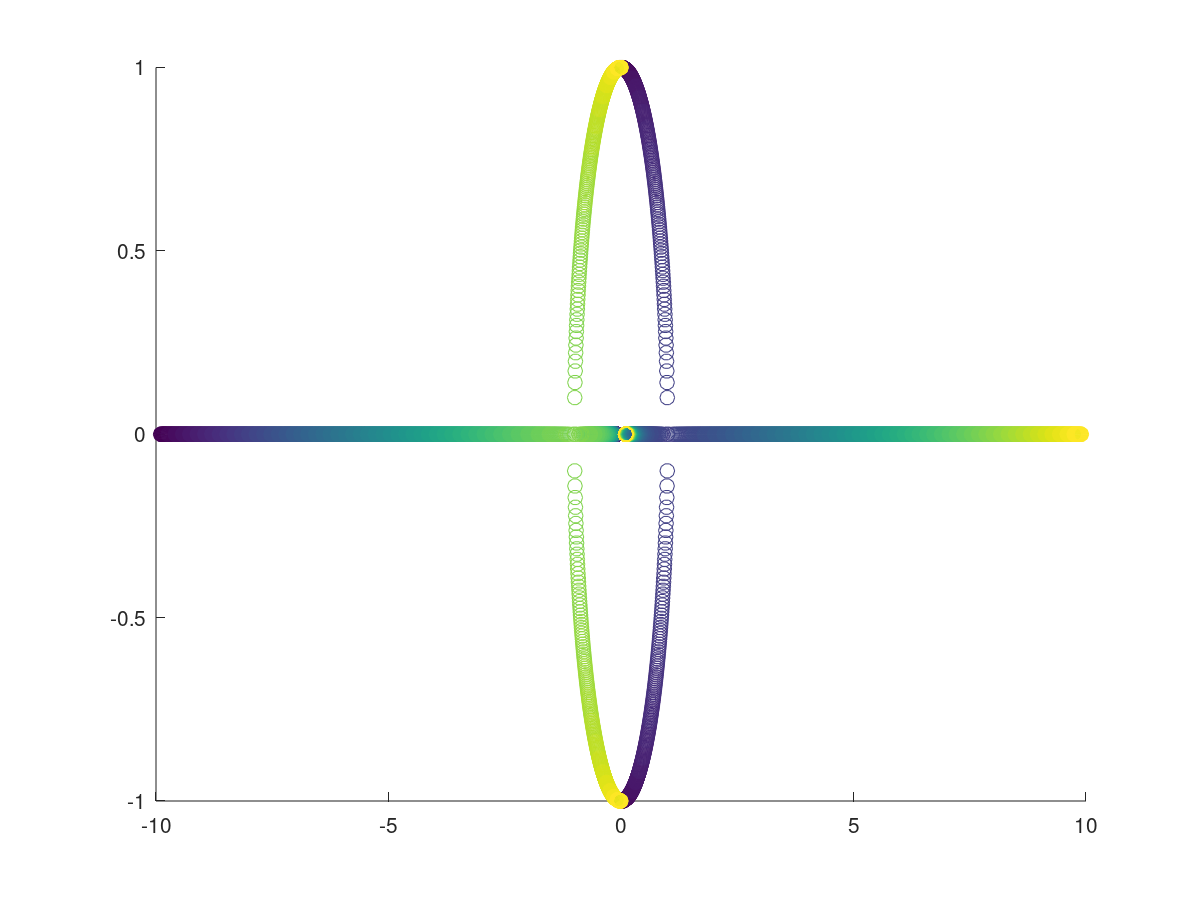
\includegraphics[width=0.8\textwidth]{ps10p1}
\end{figure}


\begin{tcolorbox}
b) For each $\lambda$, decompose the set of matrices $P \in \SL_2$ with eigenvalue $\lambda$ into $\SL_2$-conjugacy classes.
\end{tcolorbox}

\begin{proof}

We claim that for every matrix $A$ with complex eigenvalues $\lambda$ and $\overline{\lambda}$ there exists a matrix $Q \in \SL_2$ such that 
$Q^t A Q = \Lambda = \begin{pmatrix} \lambda & \\ & \overline{\lambda} \end{pmatrix}$.

Let $X = (u, v)^t$ be a unit eigenvector of $A$ with eigenvalue $\lambda$.
Then $Y = (-v,u)^t$ is also a unit eigenvector of $A$ with eigenvalues $\overline{\lambda}$. [PROVE]
Let 
$
    Q =
    \begin{pmatrix}
        u & -v \\
        v & u
    \end{pmatrix}
$, then
\begin{align*}
    Q^t A Q & = 
    \begin{pmatrix}
        u & v \\
        -v & u
    \end{pmatrix}
    \begin{pmatrix}
        a & b \\
        c & d
    \end{pmatrix}
    \begin{pmatrix}
        u & -v \\
        v & u
    \end{pmatrix}
    =
    \begin{pmatrix}
        u & v \\
        -v & u
    \end{pmatrix}
    \begin{pmatrix}
        \lambda u & -\overline{\lambda} v \\
        \lambda v & \overline{\lambda} u
    \end{pmatrix}
    \\
    & = 
    \begin{pmatrix}
        \lambda(u^2+v^2) & - \overline{\lambda} uv + \overline{\lambda} uv \\
        - \lambda uv + \lambda uv & \overline{\lambda} (v^2 + u^2)
    \end{pmatrix}
    = 
    \begin{pmatrix}
        \lambda &  \\
         & \overline{\lambda}
    \end{pmatrix}.
\end{align*}


\end{proof}

\begin{tcolorbox}
c) Determine the matrices $P \in \SL_2$ that can be obtained as $P = e^A$ for some real matrix $A$.
\end{tcolorbox}

\begin{proof}
\end{proof}

\subsection*{Problem 2}

\begin{tcolorbox}
According to Sylvester's Law, every $2 \times 2$ real symmetric matrix is congruent to exactly one of six standard types.
List them.
If we consider the operation of $\GL_2$ on $2 \times 2$ matrices by $P * A = PAP^t$, then Sylvester's Law asserts that the symmetric matrices form six orbits.
We may view the symmetric matrices as points in $\R^3$, letting $(x,y,z)$ correspond to the matrix
$
\begin{pmatrix}
    x & y \\
    y & z
\end{pmatrix}
$.
Describe the decomposition of $\R^3$ into orbits geometrically, and make a clear drawing depicting it.
\end{tcolorbox}

\begin{proof}
\end{proof}


\subsection*{Problem 3}

\begin{tcolorbox}
This problem is about the space $V$ of real polynomials in the variables $x$ and $y$.
If $f$ is a polynomial, $\partial_f$ will denote the operator 
$f \left( \frac{\partial}{\partial x}, \frac{\partial}{\partial y}) \right)$,
and $\partial_f(g)$ will denote the result of applying this operator to a polynomial $g$.

a) The rule $\bilform{f,b} = \partial_f(g)_0$ defines a bilinear form on $V$, the subscript denoting evaluation of a polynomial at the origin.
Prove that this form is symmetric and positive definite, and that the monomials $x^i y^j$ form an orthogonal basis of $V$ (not an orthonormal basis).

b) We also have the operator of multiplication by $f$, which we write as $m_f$.
So $m_f(g) = fg$.
Prove that $\partial_f$ and $m_f$ are adjoint operators.

c) When $f = x^2 + y^2$, the operator $\partial_f$ is the Laplacian, which is often written as $\Delta$.
A polynomial $h$ is harmonic if $\Delta h = 0$.
Let $H$ denote the space of harmonic polynomials.
Identify the space $H^\perp$ orthogonal to $H$ with respect to the given form.
\end{tcolorbox}

\begin{proof}
\end{proof}


\subsection*{Problem 4}

\begin{tcolorbox}
Show that the vector cross product makes $\R^3$ into a Lie algebra $L_1$.
\end{tcolorbox}

\begin{proof}
\end{proof}


\end{document}
